\section{Diskussion}

Bei der Bestimmung der differentiellen Energieverteilung fällt auf, dass die gemessenen
Kurven und somit auch die differentiellen Kurven sich stark von den erwarteten
Kurven unterscheiden. Aus der Theorie wird erwartet, dass der Auffängerstrom zumindest
bei der ersten Messreihe, bei Zimmertemperatur, auf \SI{0}{\volt} abfällt. Da das
in dieser Messung nicht der Fall war könnte sich das ermittelte Kontaktpotential,
welches in diesem Fall \SI{1.16}{\volt} ist, etwas von den realen unterscheiden.
Ein möglicher Grund für diese Ergebnisse könnte eine Fehlfunktion oder eine falsche
Einstellung des XY-Schreibers gewesen sein, da dieser öfters nicht zuverlässig
aufgezeichnet hat.

Bei der Bestimmung der Franck-Hertz-Kurve waren die Ergebnisse besser. Wenn die
ermittelte Anregungsenergie, welche U = \SI{4.746(437)}{\electronvolt} beträgt, mit den
Literaturwerten verglichen wird ergibt sich eine Abweichung von 3,14 \%.
Der Literaturwert ist in dem Fall $U_\text{lit} = \SI{4.9}{\electronvolt}$ \cite{2}.

Wie schon erwähnt unterscheidet sich die gemessene Kurve der Ionisierungsspannung
von der erwarteten Kurve aufgrund eines systematischen Fehlers. Es wird nur ein
Anstieg des Auffangstroms erwartet und danach einen plötzlichen Abfall. Den zweiten
Anstieg bei der Messung könnte durch eine erneute Ionisation der Elektronen vorliegen.

\section{Anhang}
\begin{figure}[p]
  \centering
  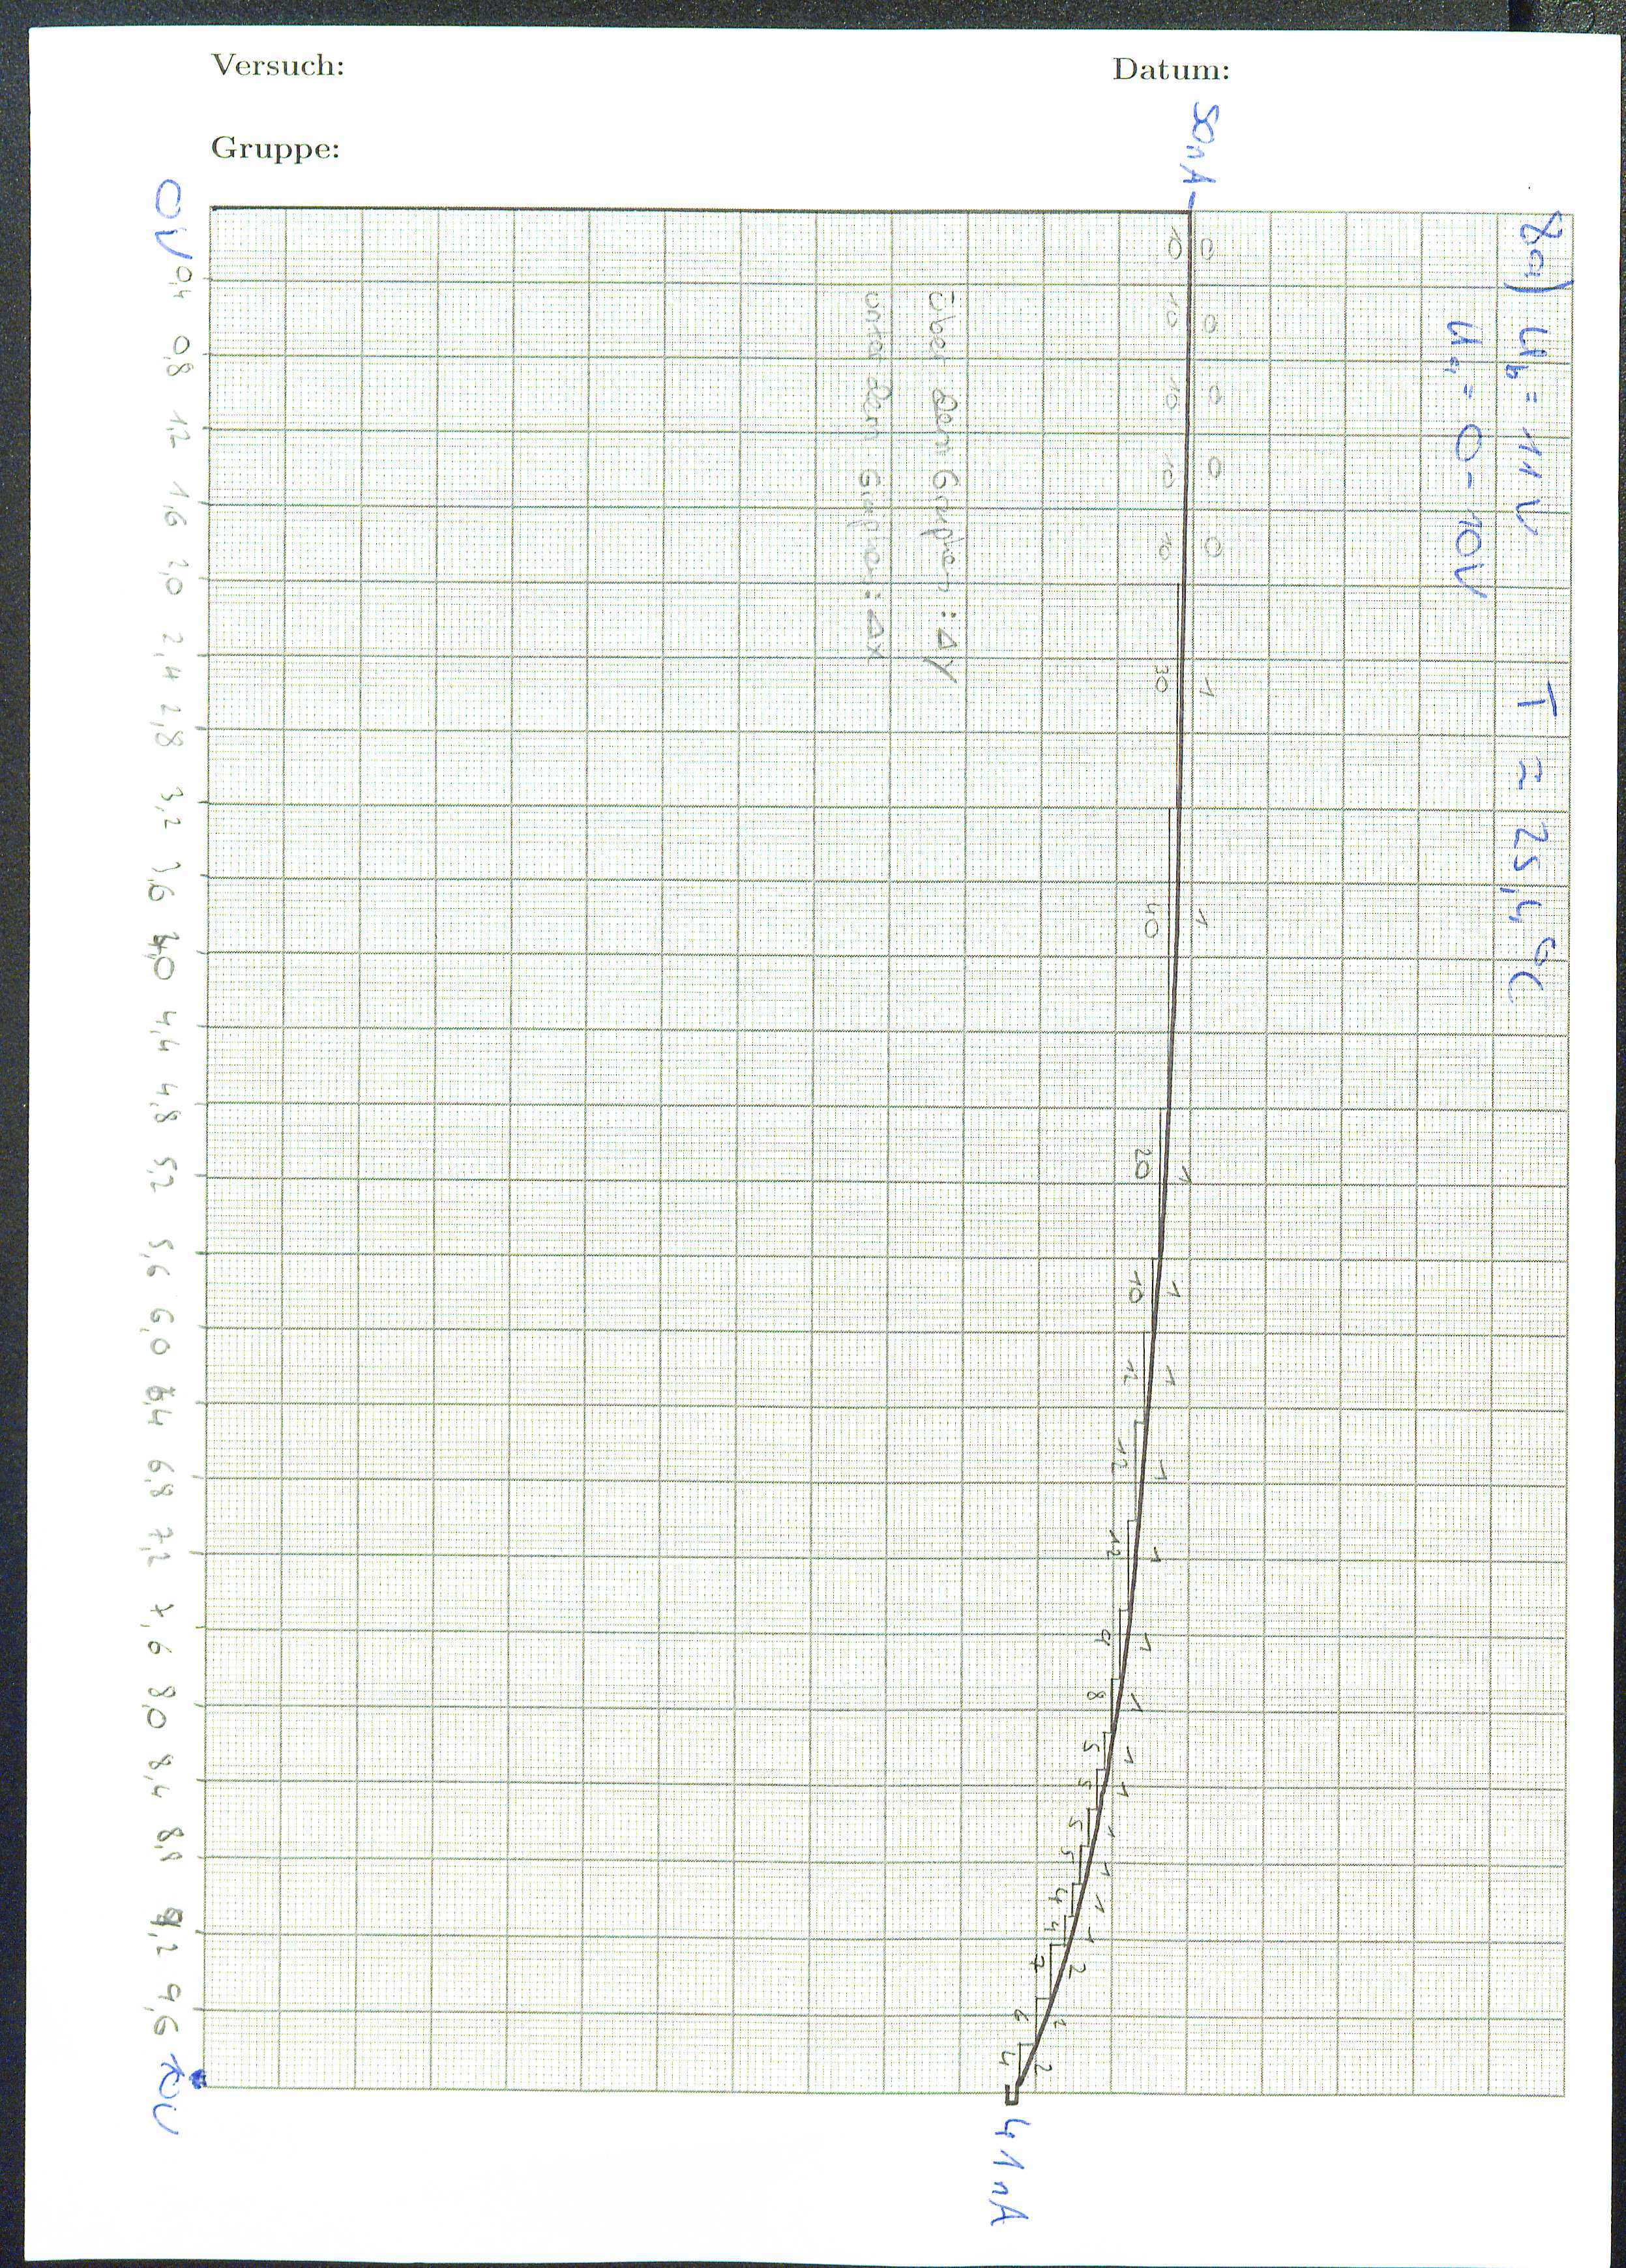
\includegraphics[width=\textwidth]{content/downKurve.jpg}
  \caption{Aufnahme zur Energieverteilung}
  \label{Bild:1}
\end{figure}
\begin{figure}[p]
  \centering
  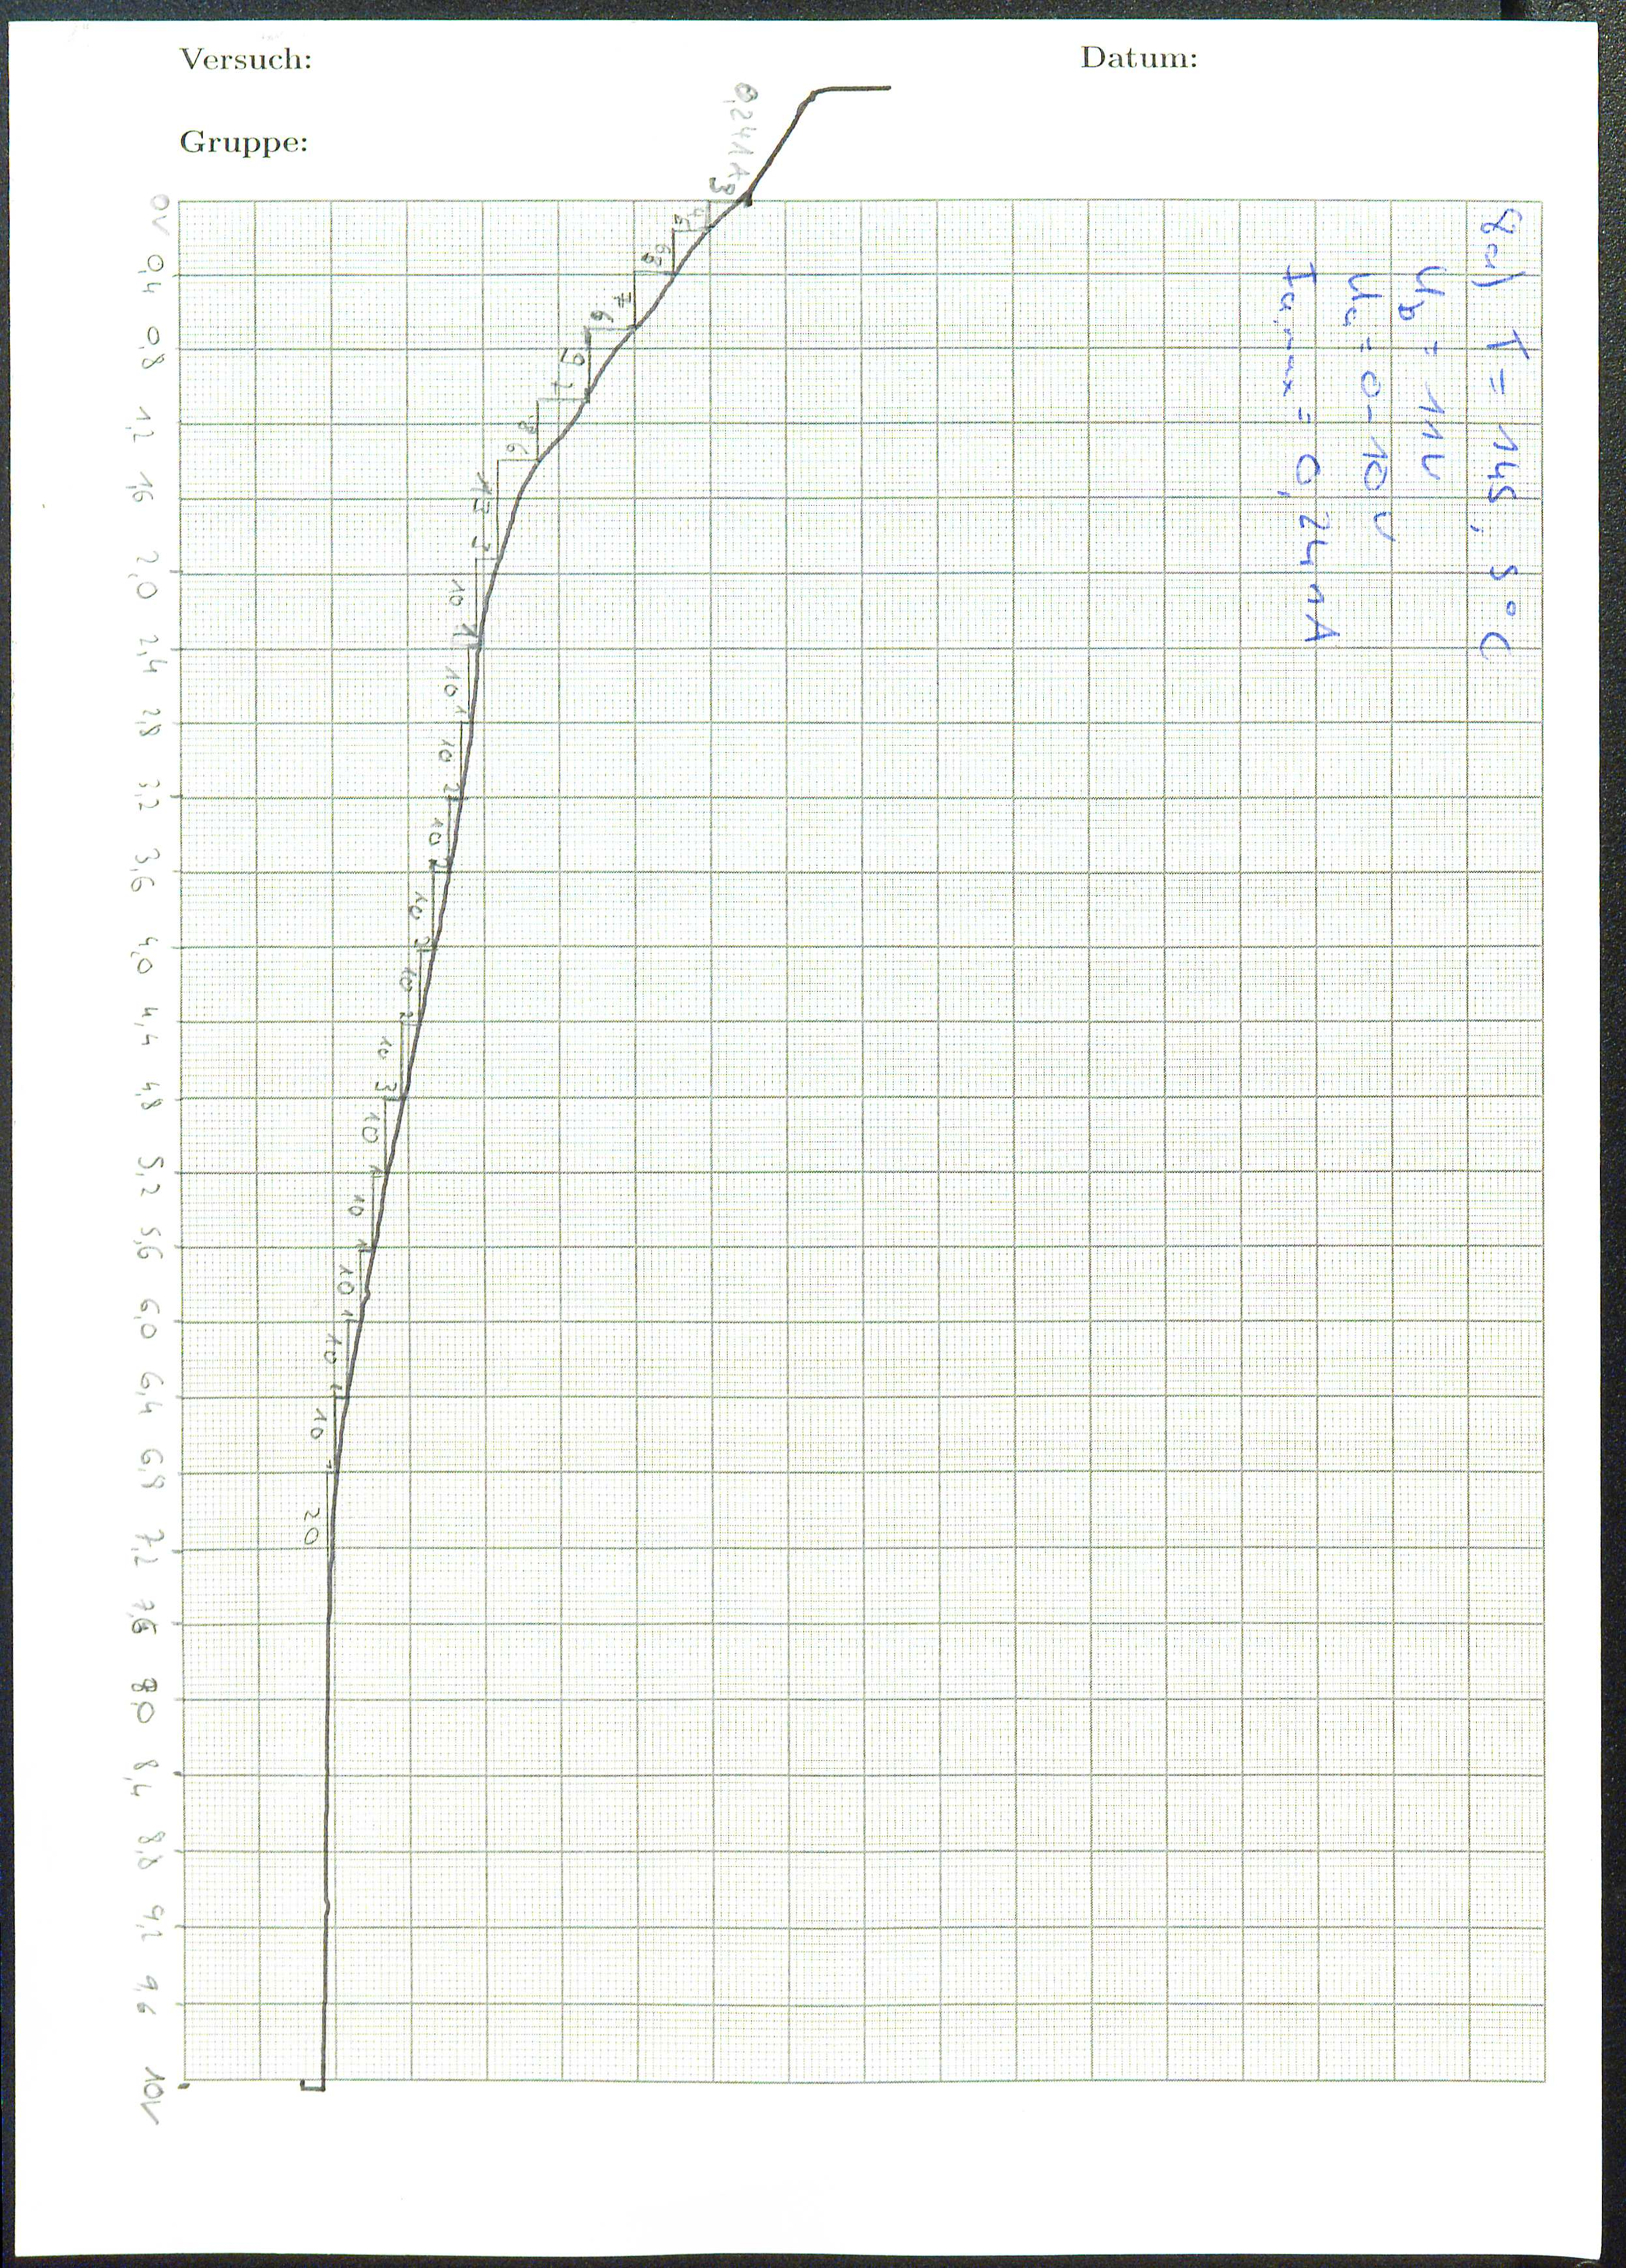
\includegraphics[width=\textwidth]{content/abKurve.jpg}
  \caption{Aufnahme zur Energieverteilung}
  \label{Bild:2}
\end{figure}
\begin{figure}[p]
  \centering
  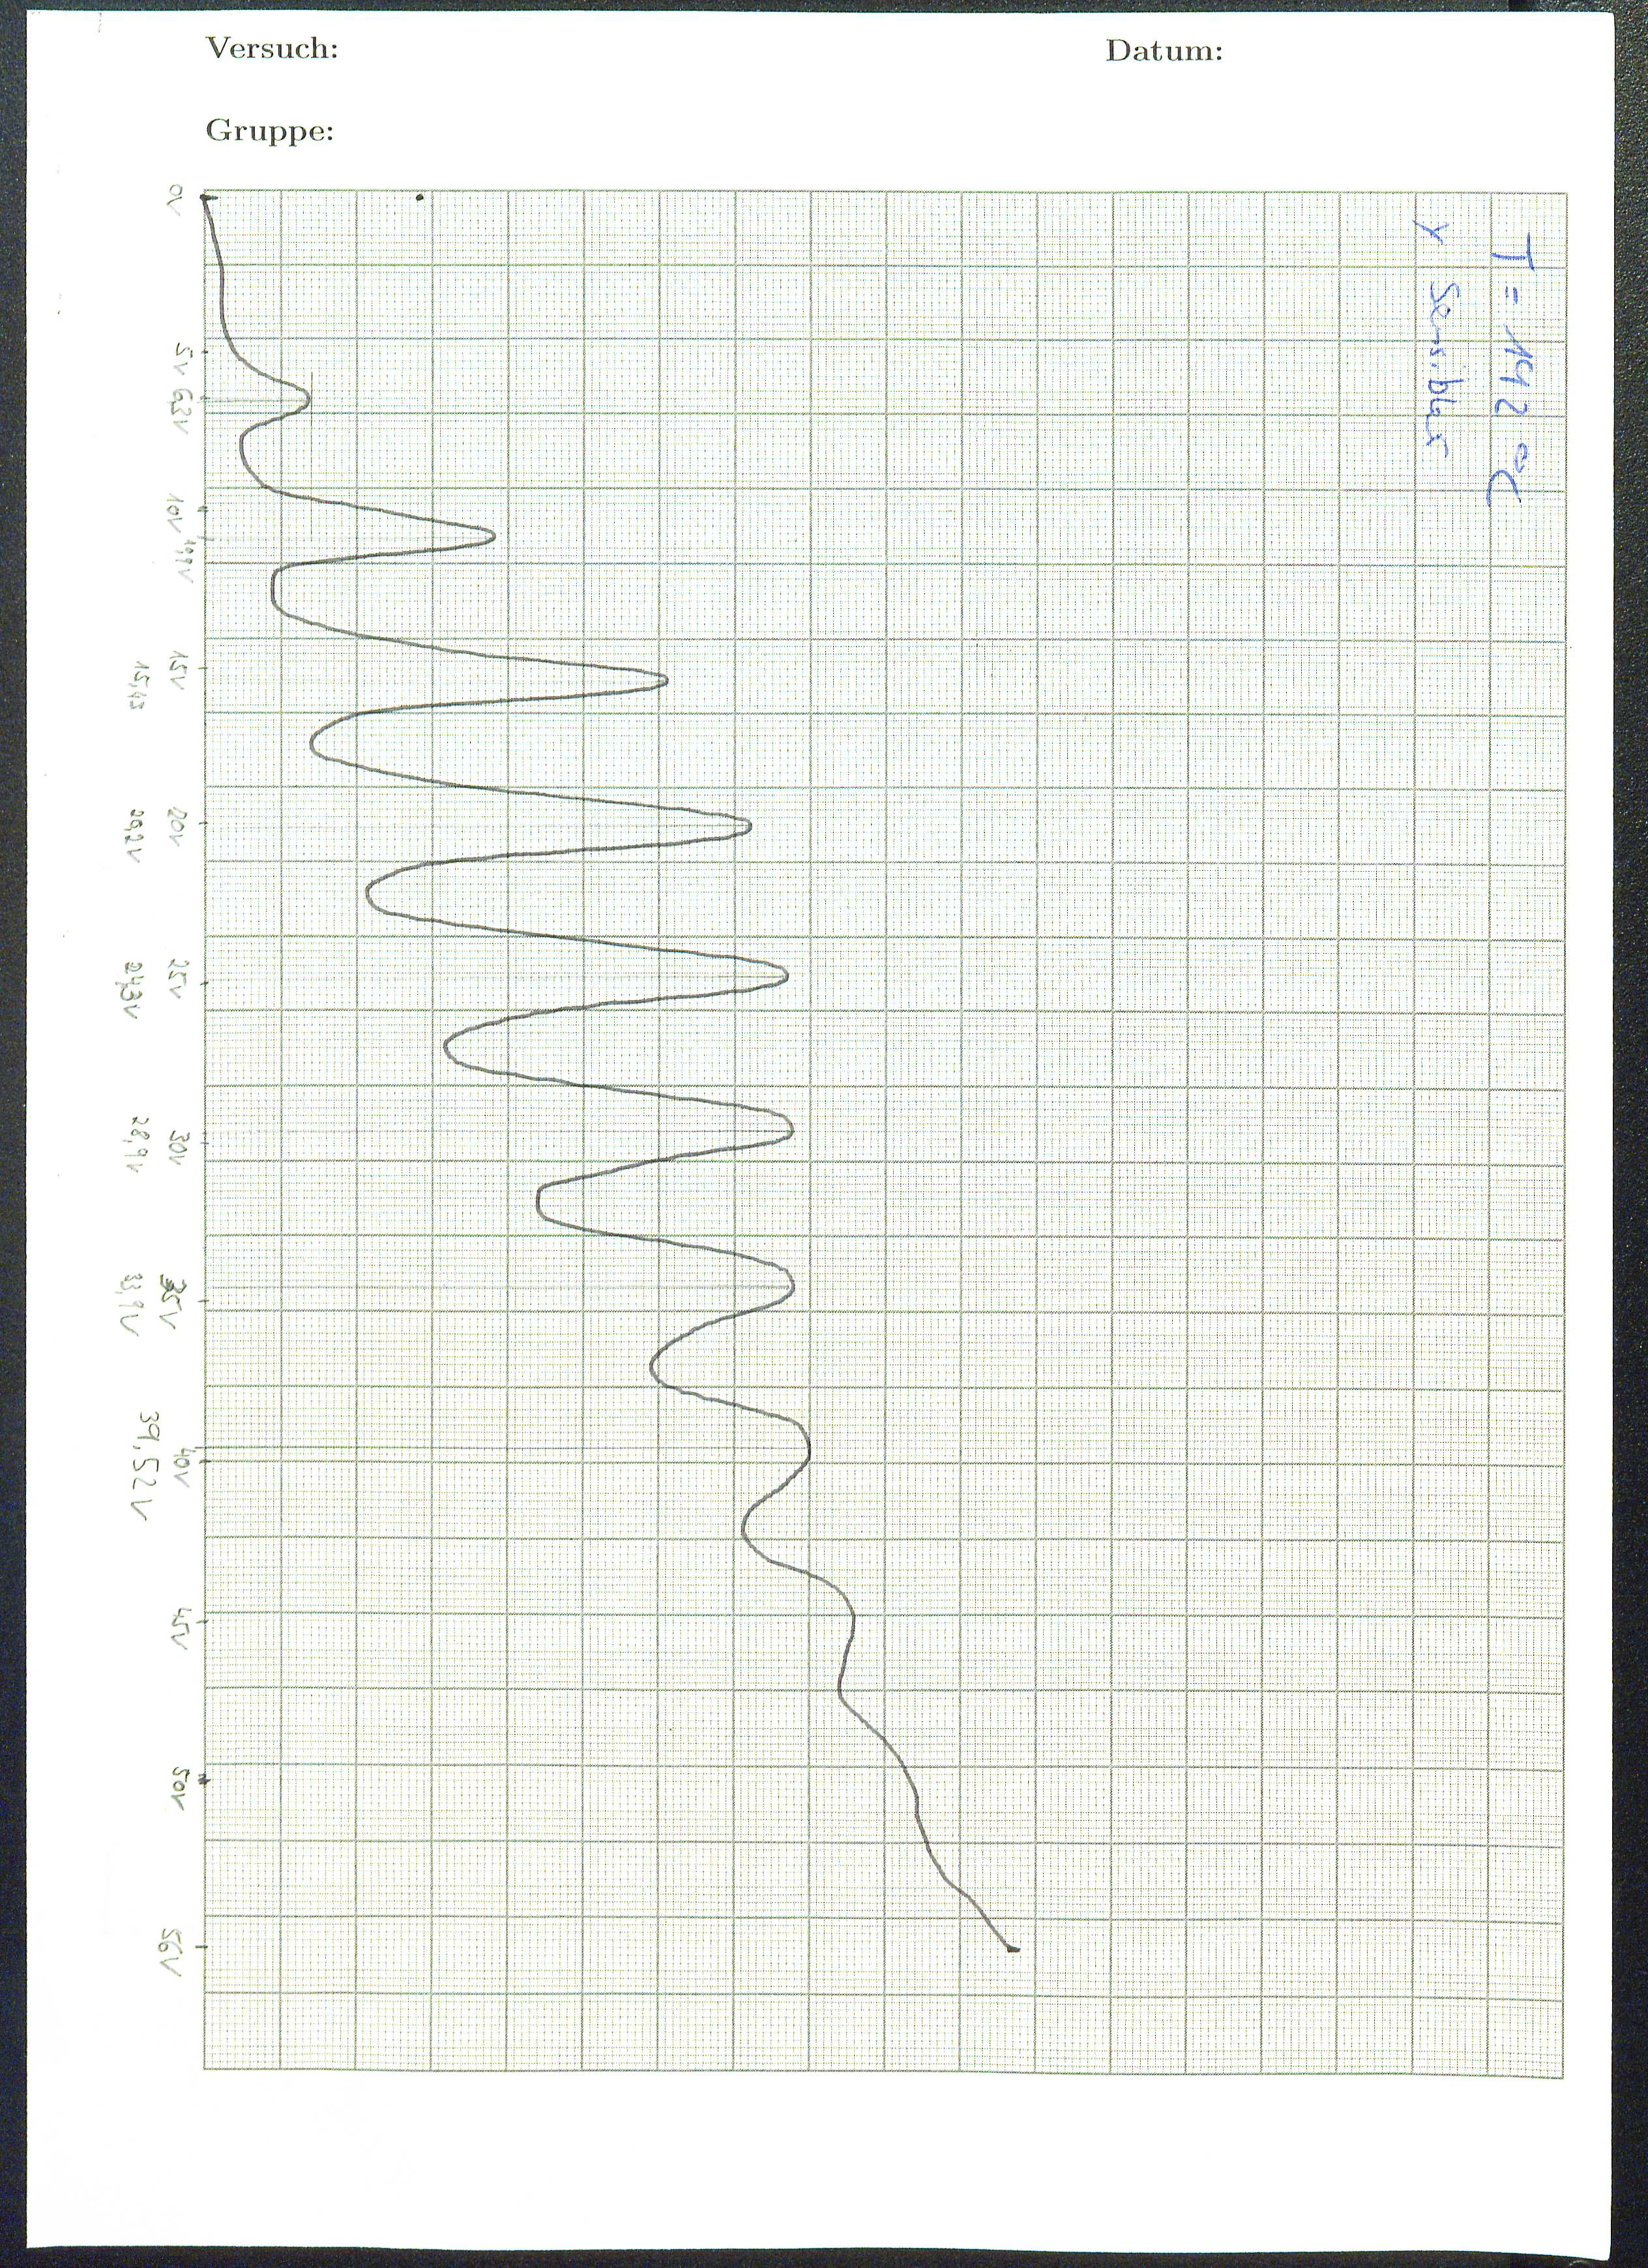
\includegraphics[width=\textwidth]{content/FHKurve.jpg}
  \caption{Aufnahme zur Franck-Hertz-Kurve}
  \label{Bild:3}
\end{figure}
\begin{figure}[p]
  \centering
  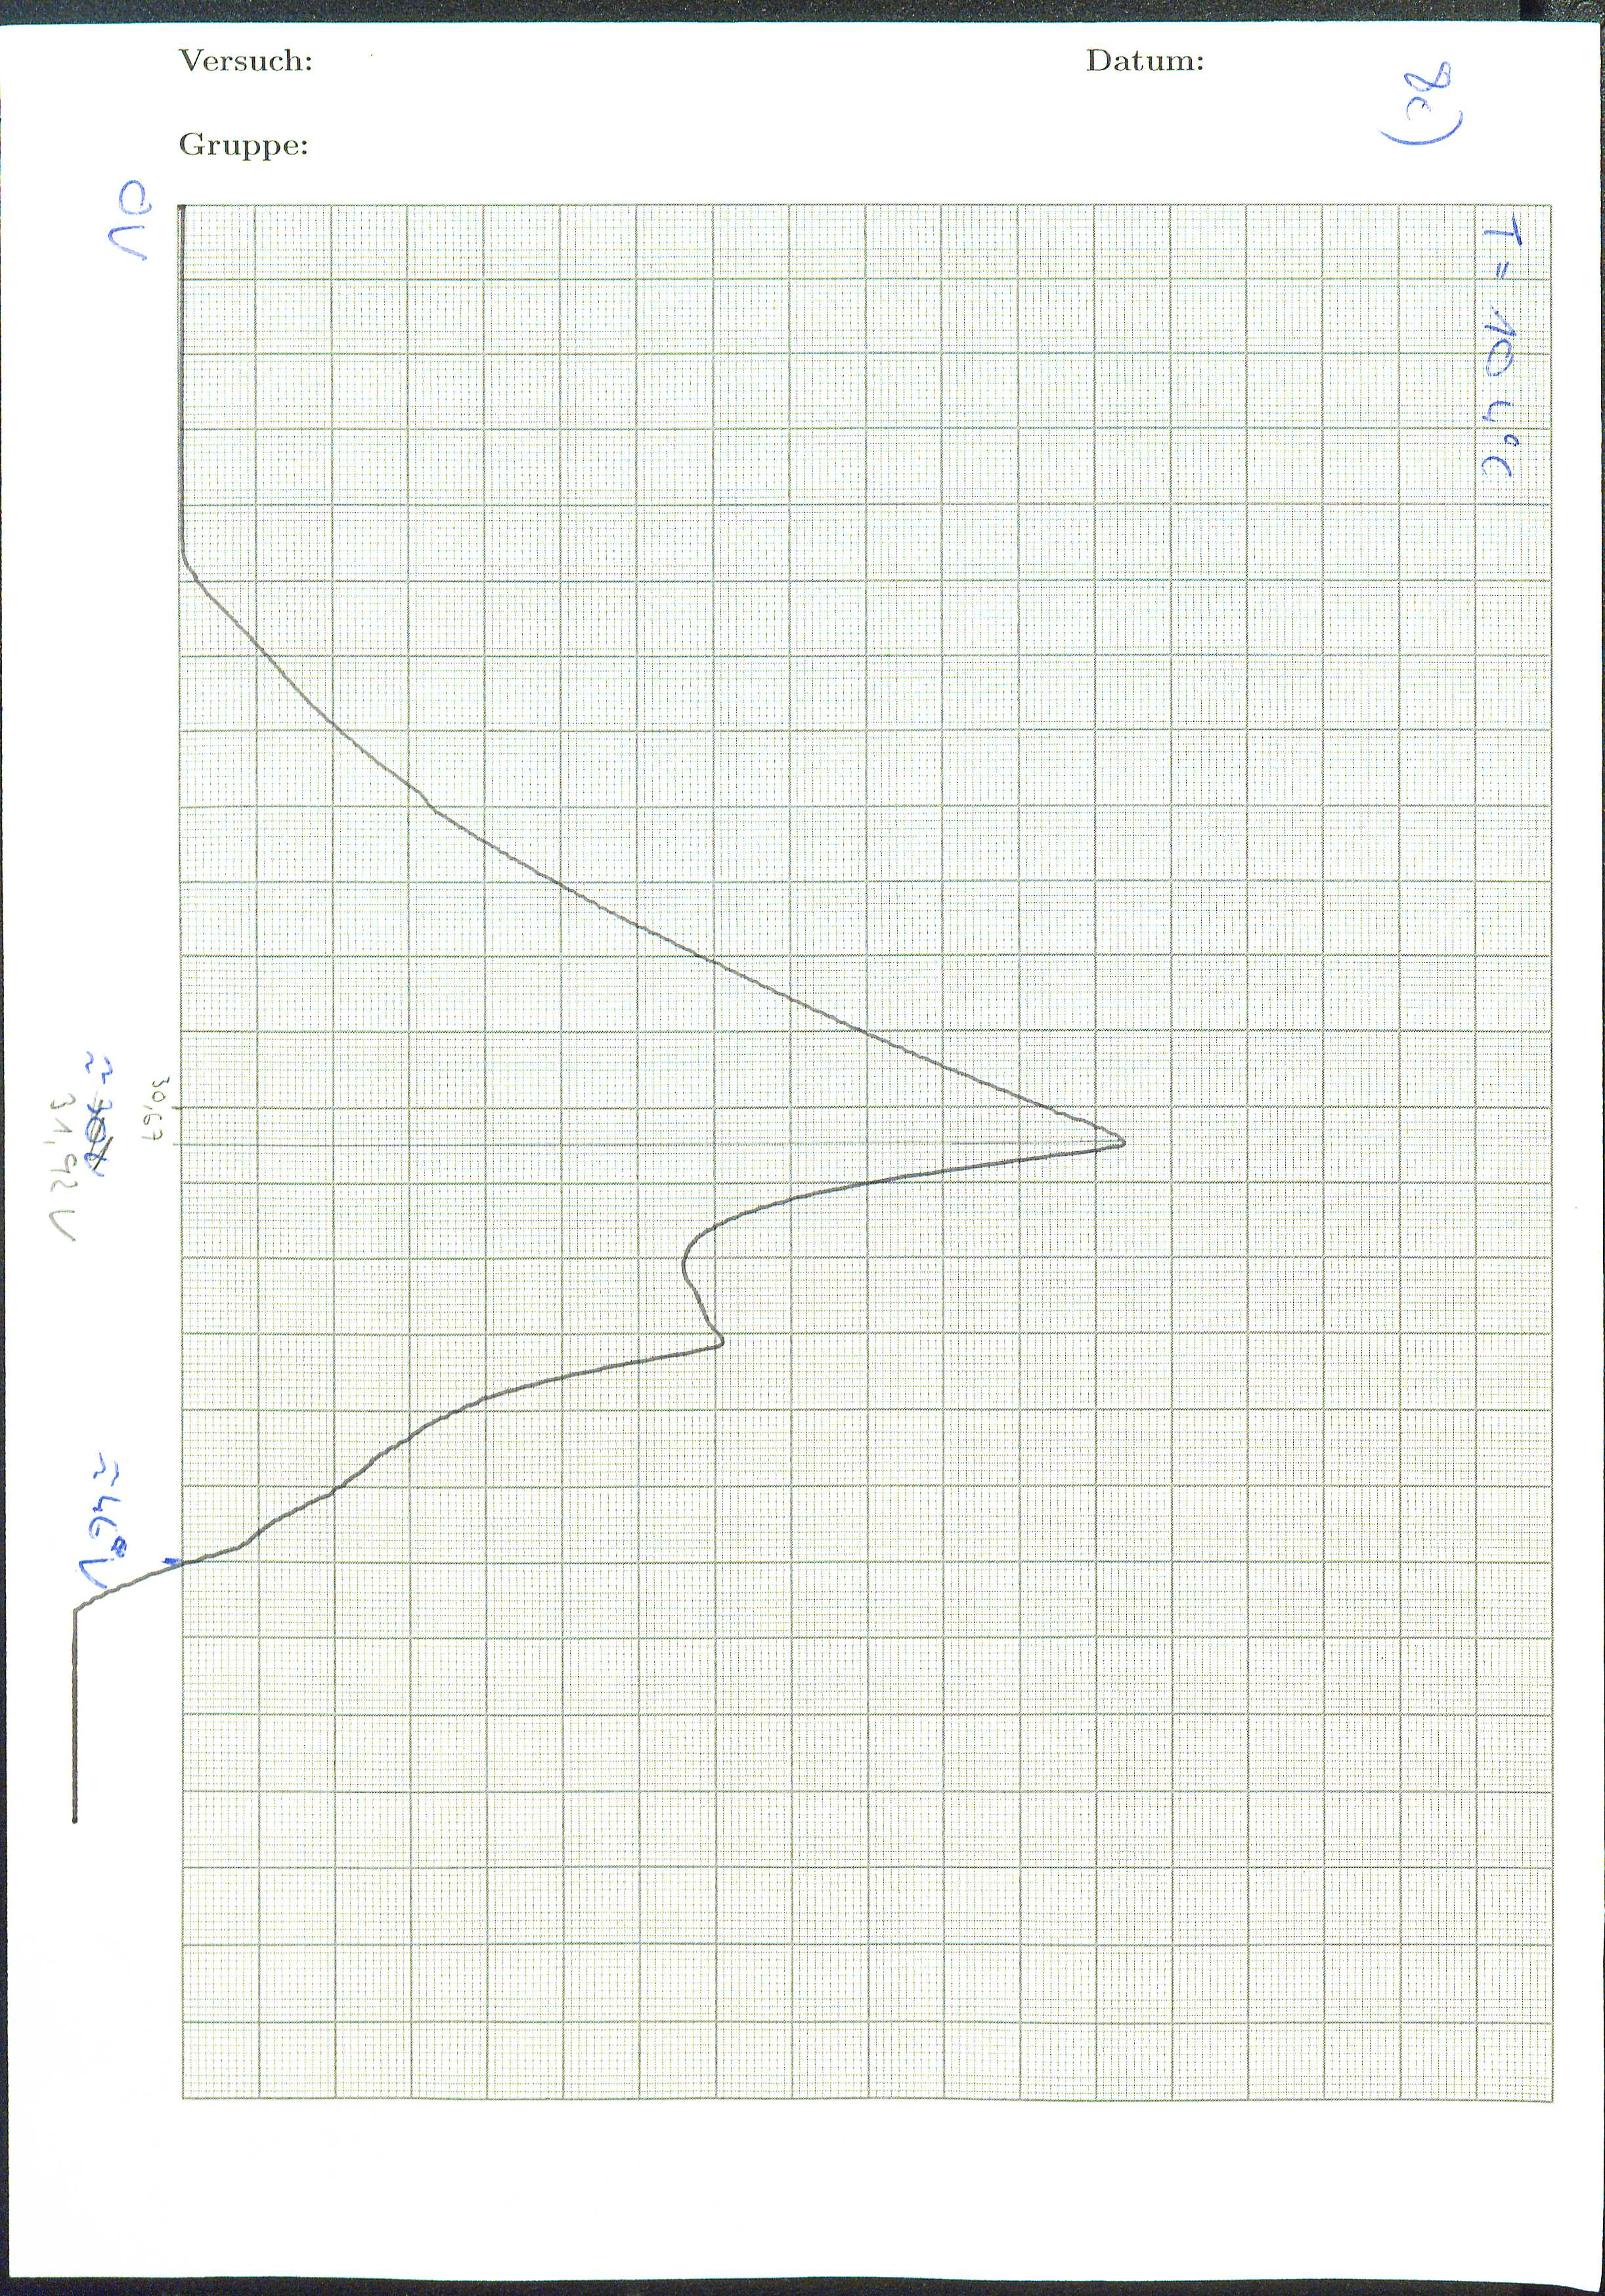
\includegraphics[width=\textwidth]{content/Ionspannung_0001.jpg}
  \caption{Aufnahme zur Bestimmung der Ionisationsenergie}
  \label{Bild:4}
\end{figure}
